\documentclass{article}

\usepackage{graphicx}

\begin{document}
	\title{Arquitectura Colonial}
	\author{Anonimo}
	\date{\today}
	\maketitle
	La \textbf{arquitectura colonial} es un estilo arquitect\'onico de una madre patria que 
	se ha incorporado a las construcciones de asentamientos o colonias. Los colonos 
	frecuentemente constru\'ian asentamientos que sintetizaban la arquitectura de sus 
	pa\'ises de origen con las caracter\'isticas de dise\~no de sus nuevas tierras, creando 
	dise\~nos h\'ibridos.\newline
  
	Durante los diversos per\'iodos coloniales -a diferencia de las ciudades europeas 
	de la \'epoca que eran una amalgama de estilos, paradigmas e ideales diferentes y 
	muchas veces opuestos- las ciudades respondieron a preceptos homogeneizadores y 
	ordenadores que expresaban c\'anones y principios que pretend\'ian instaurar una 
	forma de vida y unos mecanismos ordenadores del espacio p\'ublico y privado.\newline
  

	\subsection*{ Ciudades coloniales en Am\'erica}

	\begin{figure}[!ht]
		\centering
		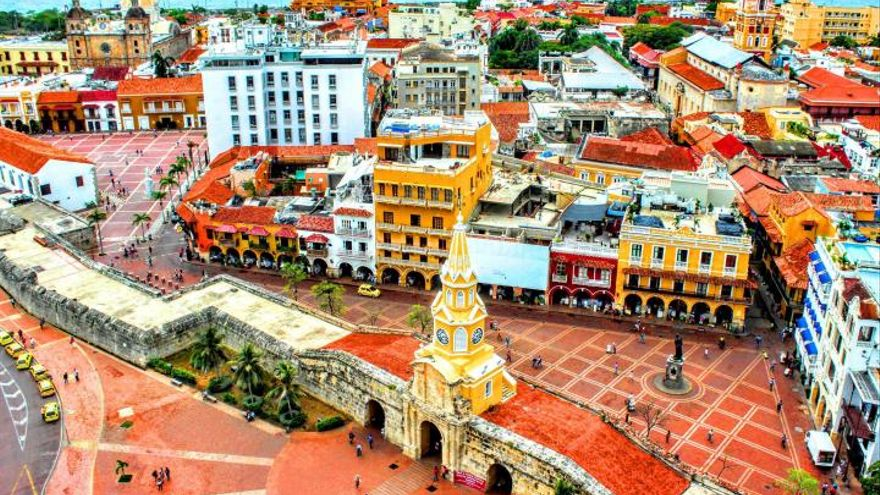
\includegraphics[width=8cm, height=6cm]{../images/cartagena_indias.jpg}
		\caption{Ciudad de Cartagena de Indias}
	\end{figure}

	\begin{figure}[!ht]
		\centering
		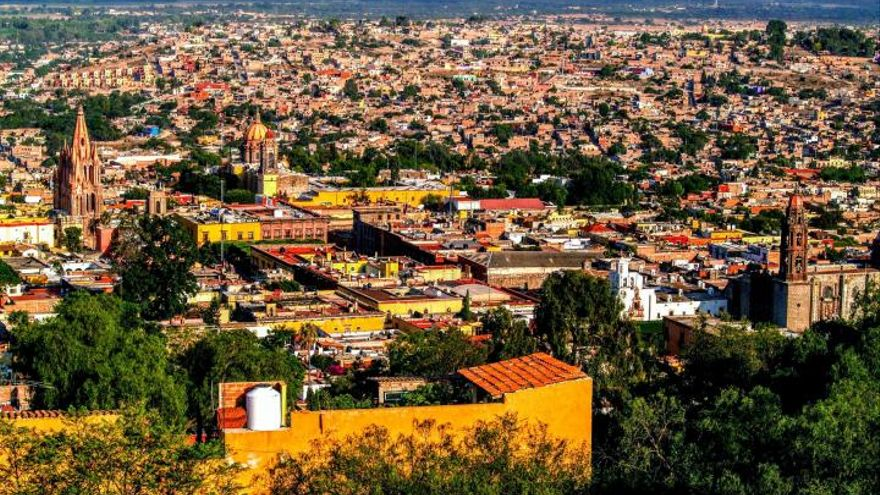
\includegraphics[width=8cm, height=6cm]{../images/san_miguel_allende.jpg}
		\caption{Ciudad de San Miguel Allende}
	\end{figure}

	\begin{figure}[!ht]
		\centering
		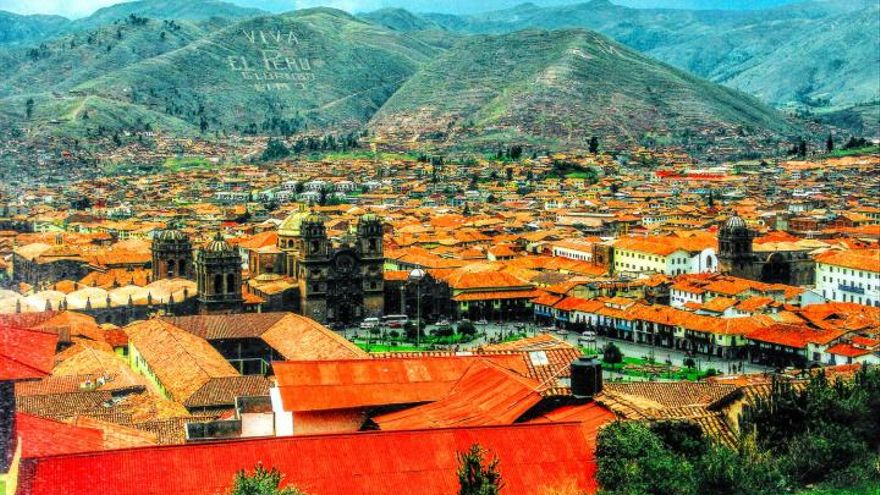
\includegraphics[width=10cm, height=7cm]{../images/cuzco.jpg}
		\caption{Ciudad de Cuzco}
	\end{figure}
\end{document}